\chapter{PK4 --- Kho \& quét}
\clearpage\begin{landscape}
\begin{figure}[H]\centering
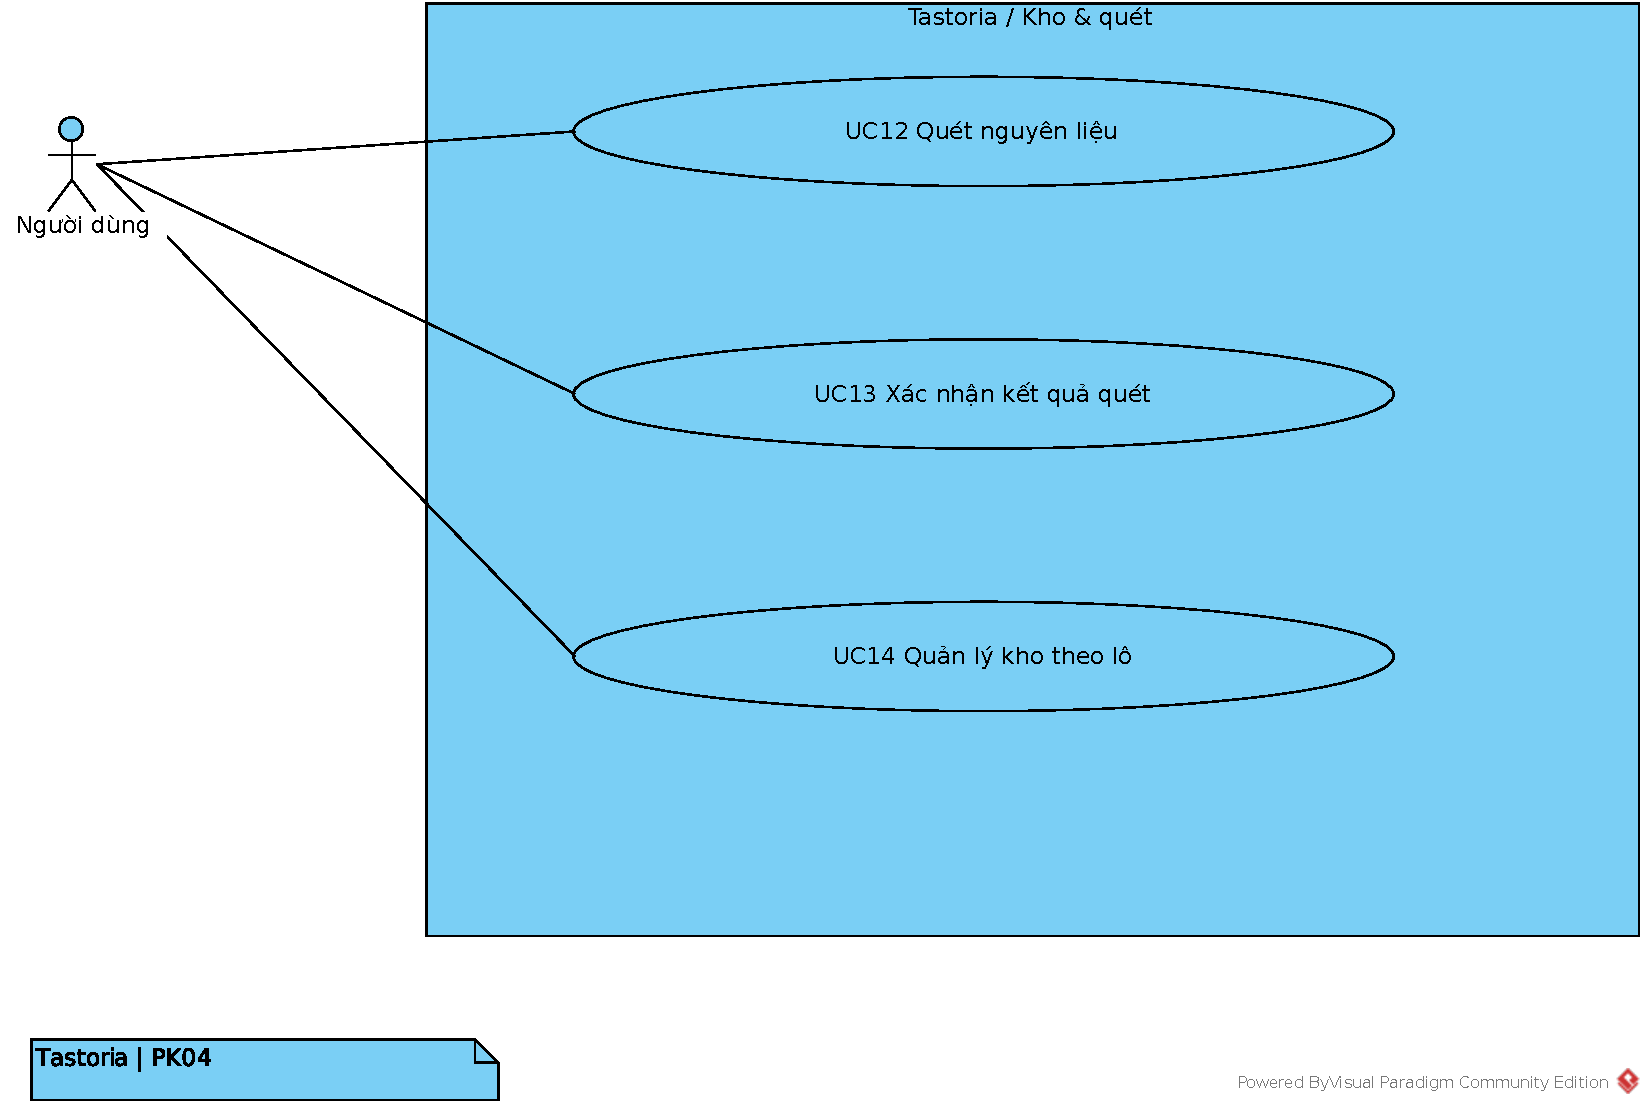
\includegraphics[width=0.96\linewidth,height=0.78\textwidth,keepaspectratio]{assets/PK04.pdf}
\caption{PK04 --- Phân rã use case}\label{fig:Phu-luc-A-Use-Cases:4}
\end{figure}
\end{landscape}\clearpage
\section{UC12 --- Quét nguyên liệu (toàn tủ hoặc đồ vừa mua)}
\subsection{Mục tiêu trong ngữ cảnh}
Người dùng (A02) chụp 1--2 ảnh tủ lạnh (chế độ "toàn tủ", {\small\texttt{fridge}}) hoặc túi đồ vừa mua (chế độ "đồ vừa mua", {\small\texttt{haul}}) để hệ thống nhận diện nguyên liệu, đếm đồ đếm được và chuẩn bị đầu vào cho đánh giá độ tươi khi có mô hình, trả về danh sách chip. Kho chưa bị ghi ở UC12; người dùng xem, sửa và xác nhận chip ở UC13 (thao tác tiếp theo).

\subsection{Phạm vi và mức}
\begin{itemize}
\item Phạm vi: hệ thống Tastoria (app, API, worker suy luận), hộp đen.
\item Mức: mục tiêu người dùng.
\item Gói: PK4 Kho \& quét.
\end{itemize}
\subsection{Tác nhân và bên liên quan (quyền lợi)}
{\footnotesize\setlength{\tabcolsep}{0pt}
\begin{longtable}{@{}L{7.850cm}@{\hspace{3mm}}L{7.850cm}@{}}
\caption{Tác nhân và bên liên quan (quyền lợi)}\\
\toprule
\textbf{Tác nhân /\allowbreak{} bên liên quan} & \textbf{Quyền lợi} \\
\midrule\endfirsthead
\multicolumn{2}{l}{\small\itshape Bảng \thetable{} (tiếp theo)}\\
\toprule
\textbf{Tác nhân /\allowbreak{} bên liên quan} & \textbf{Quyền lợi} \\
\midrule\endhead
\bottomrule\endfoot
A02 Người dùng (chính) & Có danh sách nguyên liệu nhanh (mục tiêu \ensuremath{\leq} 3 s ở server), không phải gõ tay; ảnh không bị giữ lâu hơn cần thiết. \\ \addlinespace[3pt]
Nhóm Xử lý ảnh /\allowbreak{} Học máy & Mỗi lần quét ghi đúng phiên bản bộ phát hiện, bộ phân loại, tiền xử lý; ảnh của người đã đồng ý góp ảnh được giữ để học chủ động. \\ \addlinespace[3pt]
Nhóm vận hành & Job không kẹt vô hạn; gửi lại không tạo job trùng. \\ \addlinespace[3pt]
\end{longtable}}
\subsection{Tiền điều kiện}
\begin{itemize}
\item A02 đã đăng nhập.
\item {\small\texttt{model\_\allowbreak{}\allowbreak{}deployments}} có bản {\small\texttt{detector}} đang chạy; worker đã nạp phiên ONNX.
\item App có quyền camera hoặc thư viện ảnh.
\end{itemize}
\subsection{Đảm bảo tối thiểu}
\begin{itemize}
\item Không có giao dịch kho nào được ghi trong UC12 (chỉ bước xác nhận ở UC13 mới ghi kho).
\item Một {\small\texttt{Idempotency-\allowbreak{}Key}} sinh nhiều nhất một {\small\texttt{scans}}.
\item Ảnh lưu đã bỏ metadata EXIF; ảnh không được đồng ý góp sẽ bị xoá sau 30 ngày (UC32).
\item Mọi scan kết thúc ở một trạng thái xác định: {\small\texttt{done}}, {\small\texttt{failed}} hoặc {\small\texttt{expired}} (sweeper UC34).
\end{itemize}
\subsection{Đảm bảo khi thành công}
\begin{itemize}
\item {\small\texttt{scans.\allowbreak{}status = done}}, có {\small\texttt{detector\_\allowbreak{}\allowbreak{}version\_\allowbreak{}\allowbreak{}id}}; {\small\texttt{classifier\_\allowbreak{}\allowbreak{}version\_\allowbreak{}\allowbreak{}id}} chỉ có khi triển khai bộ phân loại; có {\small\texttt{preprocess\_\allowbreak{}\allowbreak{}version}}, {\small\texttt{started\_\allowbreak{}\allowbreak{}at}}, {\small\texttt{finished\_\allowbreak{}\allowbreak{}at}}.
\item {\small\texttt{scan\_\allowbreak{}\allowbreak{}images}} có 1--2 dòng; {\small\texttt{detections}} có các khung; {\small\texttt{scan\_\allowbreak{}\allowbreak{}items}} có một chip cho mỗi nguyên liệu nhận được ({\small\texttt{origin = model}}).
\item App đang ở màn Xác nhận nguyên liệu (UC13).
\end{itemize}
\subsection{Kích hoạt}
A02 bấm "Chụp tủ lạnh" hoặc "Đồ vừa mua" ở Trang chủ.

\subsection{Kịch bản chính}
Kịch bản viết ở mức tác nhân \ensuremath{\leftrightarrow} hệ thống (hộp đen). Phân công giữa API, worker và các module ({\small\texttt{scan}}, {\small\texttt{mlops}}, {\small\texttt{catalog}}, {\small\texttt{pantry}}, {\small\texttt{privacy}}) cùng các bảng được đọc, ghi ở từng bước nằm ở {\small\texttt{docs/\allowbreak{}\allowbreak{}uml/\allowbreak{}\allowbreak{}sequence/\allowbreak{}\allowbreak{}SD01-\allowbreak{}quet-\allowbreak{}anh-\allowbreak{}bat-\allowbreak{}dong-\allowbreak{}bo.\allowbreak{}puml}} và mục 13 (Dữ liệu).

\begin{enumerate}
\item \textbf{A02} chọn chế độ (toàn tủ /\allowbreak{} đồ vừa mua) và chụp ảnh thứ nhất; tuỳ chọn chụp ảnh thứ hai và đánh dấu "ngăn khác" nếu ảnh 2 chụp ngăn khác.
\item \textbf{App} nén ảnh về cạnh dài 1.280 px JPEG, sinh {\small\texttt{Idempotency-\allowbreak{}Key}} (UUID) cho lần gửi này và gửi {\small\texttt{POST /\allowbreak{}\allowbreak{}scans}} (multipart: {\small\texttt{mode}}, 1--2 ảnh, {\small\texttt{shelf\_\allowbreak{}\allowbreak{}group}} mỗi ảnh).
\item \textbf{Hệ thống} kiểm khoá lũy đẳng, số ảnh, dung lượng, loại tệp và số điểm ảnh; xoay ảnh theo EXIF rồi lưu lại ở dạng JPEG không metadata (FR-\allowbreak{}12-\allowbreak{}02 \ldots{} FR-\allowbreak{}12-\allowbreak{}07).
\item \textbf{Hệ thống} ghi nhận lần quét ở trạng thái {\small\texttt{queued}}, đánh dấu ảnh được giữ để góp dữ liệu nếu A02 có đồng ý {\small\texttt{photo\_\allowbreak{}\allowbreak{}contribution}} (FR-\allowbreak{}12-\allowbreak{}17), đưa việc nhận diện vào hàng đợi và ghi nhớ phản hồi theo khoá lũy đẳng.
\item \textbf{Hệ thống} trả 202 kèm địa chỉ của lần quét và gợi ý thời gian hỏi lại (FR-\allowbreak{}12-\allowbreak{}08).
\item \textbf{App} hỏi trạng thái lần quét theo kiểu chờ dài (long-\allowbreak{}poll, tối đa 10 s mỗi lần; FR-\allowbreak{}12-\allowbreak{}09).
\item \textbf{Hệ thống} chạy bộ phát hiện đang triển khai trên từng ảnh và ghi các khung nhận được (FR-\allowbreak{}12-\allowbreak{}10, FR-\allowbreak{}12-\allowbreak{}11).
\item \textbf{Hệ thống (chỉ khi có mô hình; chưa triển khai ở worker hiện tại)} ước xác suất độ tươi cho khung thuộc lớp có mô hình độ tươi (FR-\allowbreak{}12-\allowbreak{}16; BR-\allowbreak{}FRESH-\allowbreak{}02).
\item \textbf{Hệ thống} quy mỗi lớp thị giác về nguyên liệu, gộp khung thành một chip cho mỗi nguyên liệu và đếm theo BR-\allowbreak{}SCAN-\allowbreak{}01 (FR-\allowbreak{}12-\allowbreak{}12, FR-\allowbreak{}12-\allowbreak{}13).
\item \textbf{Hệ thống} ghi phiên bản mô hình và tiền xử lý đã dùng, chuyển lần quét sang {\small\texttt{done}}.
\item \textbf{Hệ thống} trả cho lần hỏi đang chờ: trạng thái {\small\texttt{done}}, danh sách chip (tên nguyên liệu, số đếm, độ tin cậy cao nhất, u\_\allowbreak{}img và nhãn độ tươi), và --- với chế độ {\small\texttt{fridge}} --- danh sách lô đang {\small\texttt{in\_\allowbreak{}\allowbreak{}stock}} mà lần quét này không thấy (FR-\allowbreak{}12-\allowbreak{}18).
\item \textbf{App} mở màn Xác nhận nguyên liệu. \textbf{[chuyển sang UC13 nếu người dùng tiếp tục]}
\end{enumerate}
\subsection{Mở rộng}
\begin{itemize}
\item \textbf{1a.} A02 từ chối quyền camera: app cho chọn ảnh từ thư viện; từ chối cả hai thì hiện "Nhập tay" (thêm lô ở UC14).
\item \textbf{2a.} Mất mạng khi tải lên: app giữ ảnh và {\small\texttt{Idempotency-\allowbreak{}Key}} trong máy, tự gửi lại với đúng key đó khi có mạng; server trả lại nguyên văn phản hồi lần đầu nếu đã nhận (FR-\allowbreak{}12-\allowbreak{}06).
\item \textbf{2b.} A02 bấm "Gửi" hai lần: cùng {\small\texttt{Idempotency-\allowbreak{}Key}} \ensuremath{\rightarrow} cùng một scan.
\item \textbf{3a.} Thiếu {\small\texttt{Idempotency-\allowbreak{}Key}}: 400 {\small\texttt{idempotency\_\allowbreak{}\allowbreak{}key\_\allowbreak{}\allowbreak{}required}}.
\item \textbf{3b.} Cùng key nhưng thân khác (ảnh khác): 422 {\small\texttt{idempotency\_\allowbreak{}\allowbreak{}key\_\allowbreak{}\allowbreak{}reused}}; app sinh key mới.
\item \textbf{3c.} 0 ảnh hoặc > 2 ảnh, {\small\texttt{mode}} thiếu hay sai: 422 {\small\texttt{validation\_\allowbreak{}\allowbreak{}error}}.
\item \textbf{3d.} Ảnh > 3 MB: 413 {\small\texttt{image\_\allowbreak{}\allowbreak{}too\_\allowbreak{}\allowbreak{}large}}; tệp không phải ảnh (magic bytes): 415 {\small\texttt{unsupported\_\allowbreak{}\allowbreak{}media\_\allowbreak{}\allowbreak{}type}}; số điểm ảnh > 4096\textsuperscript{2}: 422 {\small\texttt{image\_\allowbreak{}\allowbreak{}too\_\allowbreak{}\allowbreak{}many\_\allowbreak{}\allowbreak{}pixels}}. App nén lại hoặc báo người dùng.
\item \textbf{4a.} Không có bản {\small\texttt{detector}} đang chạy: 503 {\small\texttt{model\_\allowbreak{}\allowbreak{}unavailable}} kèm {\small\texttt{Retry-\allowbreak{}After}}; không tạo scan.
\item \textbf{4b.} Hàng đợi quá dài: 503 {\small\texttt{queue\_\allowbreak{}\allowbreak{}full}} kèm {\small\texttt{Retry-\allowbreak{}After}}; không tạo scan.
\item \textbf{4c.} Lưu tệp xong nhưng đưa vào hàng đợi lỗi: giao dịch DB huỷ, tệp tạm bị xoá; 503; app gửi lại cùng key.
\item \textbf{6a.} Long-\allowbreak{}poll hết 10 s mà job chưa xong: server trả trạng thái hiện tại ({\small\texttt{queued}}/\allowbreak{}{\small\texttt{processing}}); app gọi lại, tối đa 20 s tổng; quá 20 s app hiện "Thử lại /\allowbreak{} Nhập tay" (FR-\allowbreak{}12-\allowbreak{}15).
\item \textbf{6b.} Mất mạng khi đang chờ: {\small\texttt{GET /\allowbreak{}\allowbreak{}scans/\allowbreak{}\allowbreak{}\{id\}}} lũy đẳng; app gọi lại khi có mạng.
\item \textbf{6c.} Gọi {\small\texttt{GET /\allowbreak{}\allowbreak{}scans/\allowbreak{}\allowbreak{}\{id\}}} của người khác: 404 {\small\texttt{not\_\allowbreak{}\allowbreak{}found}} (FR-\allowbreak{}12-\allowbreak{}14).
\item \textbf{7a.} Lần chạy gặp lỗi suy luận (ngoại lệ trong bộ phát hiện hoặc bộ phân loại): hệ thống đưa lần quét lại hàng đợi khi {\small\texttt{attempts}} < 3 (1 lần đầu + tối đa 2 lần thử lại); lần chạy thứ 3 vẫn lỗi thì {\small\texttt{status = failed}}, {\small\texttt{error\_\allowbreak{}\allowbreak{}code}} ghi nguyên nhân (FR-\allowbreak{}12-\allowbreak{}19). App hiện "Không nhận diện được, thử lại hoặc nhập tay".
\item \textbf{7b.} Lần chạy vượt 30 s bị cắt (FR-\allowbreak{}12-\allowbreak{}10), hoặc worker chết giữa chừng: lần quét nằm lại ở {\small\texttt{processing}}; tác vụ dọn (UC34) đưa lại hàng đợi khi {\small\texttt{attempts}} < 3, và đặt {\small\texttt{status = expired}}, {\small\texttt{error\_\allowbreak{}\allowbreak{}code = timeout}} khi {\small\texttt{attempts}} = 3 (FR-\allowbreak{}34-\allowbreak{}01, FR-\allowbreak{}34-\allowbreak{}02). App hiện như 7a.
\item \textbf{7c.} Lần quét nằm ở {\small\texttt{queued}} mà không được worker nhận (mất job): tác vụ dọn đưa lại hàng đợi; lần quét tồn tại quá 5 phút kể từ {\small\texttt{created\_\allowbreak{}\allowbreak{}at}} mà chưa rời {\small\texttt{queued}}/\allowbreak{}{\small\texttt{processing}} thì chuyển {\small\texttt{expired}} (FR-\allowbreak{}34-\allowbreak{}11).
\item \textbf{8a.} Lớp không có mô hình độ tươi hoặc không có bản {\small\texttt{freshness}} đang chạy: các cột {\small\texttt{p\_\allowbreak{}\allowbreak{}*}} để NULL; {\small\texttt{classifier\_\allowbreak{}\allowbreak{}version\_\allowbreak{}\allowbreak{}id}} NULL; độ gấp lô sau này dùng u = u\_\allowbreak{}time (BR-\allowbreak{}FRESH-\allowbreak{}02).
\item \textbf{9a.} Không phát hiện khung nào: {\small\texttt{status = done}} với danh sách chip rỗng; app hiện "Chưa thấy nguyên liệu nào" và nút "Thêm" (UC13).
\item \textbf{9b.} Nhiều lớp quy về cùng một nguyên liệu: gộp vào một chip.
\item \textbf{9c.} Ảnh mờ, tối (chất lượng thấp): chip có độ tin cậy thấp hiện nhạt hơn ở UC13; không chặn quét.
\item \textbf{11a.} Chế độ {\small\texttt{haul}}: không trả danh sách lô "không thấy" (BR-\allowbreak{}PANTRY-\allowbreak{}03).
\item \textbf{*a.} A02 rời màn hình khi scan đang chạy: scan tiếp tục; lần mở sau app lấy lại theo {\small\texttt{scan\_\allowbreak{}\allowbreak{}id}} đã lưu.
\item \textbf{*b.} Lỗi hệ thống không lường: 500 {\small\texttt{problem+json}} có {\small\texttt{request\_\allowbreak{}\allowbreak{}id}}; scan không đổi trạng thái.
\end{itemize}
\subsection{Ghi chú đối chiếu của báo cáo}
Phạm vi UC12 dừng ở kết quả nhận diện; UC13 là mục tiêu xác nhận riêng. Không dùng include để mô tả chuyển màn hình. Bộ phân loại độ tươi chưa được triển khai trong worker hiện tại; classifier\_\allowbreak{}version\_\allowbreak{}id có thể rỗng, không coi xác suất độ tươi là hậu điều kiện bắt buộc của phiên bản đang chạy.

\textbf{Nguồn:} {\small\texttt{Tastoria/\allowbreak{}\allowbreak{}docs/\allowbreak{}\allowbreak{}sad/\allowbreak{}\allowbreak{}use-\allowbreak{}cases/\allowbreak{}\allowbreak{}UC12.\allowbreak{}md}}. Mã nghiệp vụ: BR-\allowbreak{}SCAN-\allowbreak{}01, BR-\allowbreak{}PANTRY-\allowbreak{}03, BR-\allowbreak{}FRESH-\allowbreak{}02, BR-\allowbreak{}RETAIN-\allowbreak{}01, BR-\allowbreak{}CONSENT-\allowbreak{}01.

\textbf{Dữ liệu liên quan:} {\small\texttt{scans}}, {\small\texttt{scan\_\allowbreak{}\allowbreak{}images}}, {\small\texttt{scan\_\allowbreak{}\allowbreak{}items}}, {\small\texttt{detections}}, {\small\texttt{idempotency\_\allowbreak{}\allowbreak{}keys}}, {\small\texttt{model\_\allowbreak{}\allowbreak{}deployments}}, {\small\texttt{model\_\allowbreak{}\allowbreak{}versions}}, {\small\texttt{model\_\allowbreak{}\allowbreak{}version\_\allowbreak{}\allowbreak{}classes}}, {\small\texttt{vision\_\allowbreak{}\allowbreak{}classes}}, {\small\texttt{vision\_\allowbreak{}\allowbreak{}class\_\allowbreak{}\allowbreak{}ingredients}}, {\small\texttt{ingredients}}, {\small\texttt{pantry\_\allowbreak{}\allowbreak{}lots}}, {\small\texttt{v\_\allowbreak{}\allowbreak{}current\_\allowbreak{}\allowbreak{}consents}}.

\textbf{Điểm giao tiếp:} {\small\texttt{POST /\allowbreak{}\allowbreak{}scans}}; {\small\texttt{GET /\allowbreak{}\allowbreak{}scans/\allowbreak{}\allowbreak{}\{id\}}}.

\section{UC13 --- Xác nhận và sửa kết quả quét}
\subsection{Mục tiêu trong ngữ cảnh}
Sau khi UC12 trả danh sách chip, người dùng (A02) sửa những gì mô hình nhận sai (đổi tên, sửa số, chọn mức ít/\allowbreak{}vừa/\allowbreak{}nhiều, thêm đồ bị sót, xoá đồ thừa), xác nhận các chip ở mức "kiểm tra trước khi dùng", rồi bấm xác nhận để đưa vào kho. Chỉ bước xác nhận mới ghi kho; mọi sửa chip trước đó là dữ liệu nháp và là tín hiệu chọn ảnh cho học chủ động.

\subsection{Phạm vi và mức}
\begin{itemize}
\item Phạm vi: hệ thống Tastoria, hộp đen.
\item Mức: mục tiêu con (subfunction), được UC12 include; cũng mở trực tiếp từ một scan {\small\texttt{done}} chưa xác nhận.
\item Gói: PK4 Kho \& quét.
\end{itemize}
\subsection{Tác nhân và bên liên quan (quyền lợi)}
{\footnotesize\setlength{\tabcolsep}{0pt}
\begin{longtable}{@{}L{7.850cm}@{\hspace{3mm}}L{7.850cm}@{}}
\caption{Tác nhân và bên liên quan (quyền lợi)}\\
\toprule
\textbf{Tác nhân /\allowbreak{} bên liên quan} & \textbf{Quyền lợi} \\
\midrule\endfirsthead
\multicolumn{2}{l}{\small\itshape Bảng \thetable{} (tiếp theo)}\\
\toprule
\textbf{Tác nhân /\allowbreak{} bên liên quan} & \textbf{Quyền lợi} \\
\midrule\endhead
\bottomrule\endfoot
A02 Người dùng (chính) & Sửa nhanh bằng chạm; kho phản ánh đúng thứ đang có; không bị đưa đồ đáng ngờ vào kho mà không biết. \\ \addlinespace[3pt]
Người ăn cùng & Đồ ở mức "kiểm tra" không vào kho khả dụng khi chưa được người dùng xác nhận. \\ \addlinespace[3pt]
Nhóm Học máy /\allowbreak{} Xử lý ảnh & Sửa chip (đổi nhãn, sửa số, xoá) được lưu kèm nhãn gốc để chọn ảnh học chủ động (với người đã đồng ý góp ảnh). \\ \addlinespace[3pt]
\end{longtable}}
\subsection{Tiền điều kiện}
\begin{itemize}
\item A02 đã đăng nhập; scan thuộc A02 và ở {\small\texttt{status = done}}.
\end{itemize}
\subsection{Đảm bảo tối thiểu}
\begin{itemize}
\item Không có dòng {\small\texttt{pantry\_\allowbreak{}\allowbreak{}lots}}/\allowbreak{}{\small\texttt{pantry\_\allowbreak{}\allowbreak{}transactions}} nào được tạo hay đổi trước khi xác nhận thành công (BR-\allowbreak{}SCAN-\allowbreak{}02).
\item Xác nhận hoặc ghi toàn bộ kho của scan trong một giao dịch, hoặc không ghi gì.
\item Xác nhận gửi lại nhiều lần chỉ ghi kho một lần.
\end{itemize}
\subsection{Đảm bảo khi thành công}
\begin{itemize}
\item {\small\texttt{scans.\allowbreak{}status = confirmed}}, {\small\texttt{confirmed\_\allowbreak{}\allowbreak{}at}} có giá trị.
\item Mỗi chip không bị xoá tạo một lô mới hoặc cập nhật quan sát của lô hiện có theo FR-\allowbreak{}13-\allowbreak{}13 đến FR-\allowbreak{}13-\allowbreak{}16; lô {\small\texttt{in\_\allowbreak{}\allowbreak{}stock}} không thấy ở chế độ {\small\texttt{fridge}} chuyển {\small\texttt{not\_\allowbreak{}\allowbreak{}seen}}.
\item Mọi chip có {\small\texttt{user\_\allowbreak{}\allowbreak{}action}} phản ánh thao tác của người dùng.
\end{itemize}
\subsection{Kích hoạt}
\begin{itemize}
\item Include từ UC12 bước 12; hoặc
\item A02 mở lại một scan {\small\texttt{done}} từ thông báo "Bạn có kết quả quét chưa xác nhận" ở Trang chủ.
\end{itemize}
\subsection{Kịch bản chính}
Kịch bản viết ở mức tác nhân \ensuremath{\leftrightarrow} hệ thống (hộp đen). Lời gọi giữa module {\small\texttt{scan}}, {\small\texttt{pantry}}, {\small\texttt{catalog}} và Unit of Work ở bước 12--13 nằm ở {\small\texttt{docs/\allowbreak{}\allowbreak{}uml/\allowbreak{}\allowbreak{}sequence/\allowbreak{}\allowbreak{}SD02-\allowbreak{}xac-\allowbreak{}nhan-\allowbreak{}quet.\allowbreak{}puml}}.

\begin{enumerate}
\item \textbf{App} hiện màn Xác nhận nguyên liệu từ dữ liệu {\small\texttt{GET /\allowbreak{}\allowbreak{}scans/\allowbreak{}\allowbreak{}\{id\}}}: chip theo nhóm thực phẩm, mỗi chip có tên, số đếm hoặc mức lượng, nhãn độ tươi (chữ kèm chấm màu); chip độ tin cậy thấp hiện nhạt hơn; nhóm "Cần kiểm tra" đặt trên cùng.
\item \textbf{A02} chạm một chip bị nhận sai tên, tìm nguyên liệu đúng.
\item \textbf{App} gọi {\small\texttt{GET /\allowbreak{}\allowbreak{}ingredients?q=}} (tìm theo {\small\texttt{name\_\allowbreak{}\allowbreak{}vi}} và {\small\texttt{ingredient\_\allowbreak{}\allowbreak{}synonyms}}), A02 chọn kết quả.
\item \textbf{App} gửi {\small\texttt{PATCH /\allowbreak{}\allowbreak{}scans/\allowbreak{}\allowbreak{}\{id\}/\allowbreak{}\allowbreak{}items/\allowbreak{}\allowbreak{}\{itemId\}}} với {\small\texttt{ingredient\_\allowbreak{}\allowbreak{}id}} mới. \textbf{Hệ thống} lưu {\small\texttt{original\_\allowbreak{}\allowbreak{}ingredient\_\allowbreak{}\allowbreak{}id}}, đặt {\small\texttt{user\_\allowbreak{}\allowbreak{}action = relabeled}}.
\item \textbf{A02} sửa số trứng từ 4 thành 6; chọn mức "vừa" cho chip rau muống. \textbf{App} gửi {\small\texttt{PATCH}} tương ứng; \textbf{hệ thống} ghi {\small\texttt{final\_\allowbreak{}\allowbreak{}count}} /\allowbreak{} {\small\texttt{qty\_\allowbreak{}\allowbreak{}level}}, {\small\texttt{user\_\allowbreak{}\allowbreak{}action = edited}}.
\item \textbf{A02} bấm "Thêm" để thêm đồ mô hình bỏ sót. \textbf{App} gửi {\small\texttt{POST /\allowbreak{}\allowbreak{}scans/\allowbreak{}\allowbreak{}\{id\}/\allowbreak{}\allowbreak{}items}}; \textbf{hệ thống} tạo chip {\small\texttt{origin = user\_\allowbreak{}\allowbreak{}added}}.
\item \textbf{A02} xoá một chip thừa. \textbf{App} gửi {\small\texttt{DELETE /\allowbreak{}\allowbreak{}scans/\allowbreak{}\allowbreak{}\{id\}/\allowbreak{}\allowbreak{}items/\allowbreak{}\allowbreak{}\{itemId\}}}; \textbf{hệ thống} đặt {\small\texttt{user\_\allowbreak{}\allowbreak{}action = deleted}} (chip của mô hình) hoặc xoá dòng (chip người dùng thêm).
\item \textbf{A02} xem chip "Cần kiểm tra trước khi dùng", chọn "Vẫn dùng được" (hoặc xoá chip). \textbf{App} gửi {\small\texttt{PATCH}} với {\small\texttt{user\_\allowbreak{}\allowbreak{}freshness}}.
\item Ở chế độ {\small\texttt{fridge}}, \textbf{app} hiện danh sách "Lần này không thấy" (các lô {\small\texttt{in\_\allowbreak{}\allowbreak{}stock}} không có chip) với chú thích "Sẽ được đánh dấu chưa thấy; bạn xác nhận ở Kho".
\item \textbf{A02} bấm "Đưa vào kho".
\item \textbf{App} gửi {\small\texttt{POST /\allowbreak{}\allowbreak{}scans/\allowbreak{}\allowbreak{}\{id\}/\allowbreak{}\allowbreak{}confirm}}.
\item \textbf{Hệ thống} kiểm lần quét đang {\small\texttt{done}} và mọi chip đủ điều kiện xác nhận (FR-\allowbreak{}13-\allowbreak{}09, FR-\allowbreak{}13-\allowbreak{}11); quy lượng mỗi chip về khoảng gam [g\_\allowbreak{}min, g\_\allowbreak{}max] (BR-\allowbreak{}QTY-\allowbreak{}02).
\item \textbf{Hệ thống} ghi kho trong một giao dịch: tạo lô mới hoặc ghi quan sát cho lô hiện có, với chế độ {\small\texttt{fridge}} đánh dấu {\small\texttt{not\_\allowbreak{}\allowbreak{}seen}} các lô {\small\texttt{in\_\allowbreak{}\allowbreak{}stock}} không thấy (BR-\allowbreak{}PANTRY-\allowbreak{}03), rồi chuyển lần quét sang {\small\texttt{confirmed}} (BR-\allowbreak{}SCAN-\allowbreak{}02).
\item \textbf{App} hiện tóm tắt "Đã thêm n món vào kho" và nút "Ra mâm cơm" (UC15). Use case kết thúc.
\end{enumerate}
\subsection{Mở rộng}
\begin{itemize}
\item \textbf{1a.} Scan không ở {\small\texttt{done}} ({\small\texttt{queued}}, {\small\texttt{processing}}): app quay về màn chờ của UC12. {\small\texttt{failed}}/\allowbreak{}{\small\texttt{expired}}: app hiện "Không nhận diện được" và nút "Quét lại" /\allowbreak{} "Nhập tay" (UC14).
\item \textbf{1b.} A02 muốn xem ảnh gốc để đối chiếu: app gọi {\small\texttt{GET /\allowbreak{}\allowbreak{}scans/\allowbreak{}\allowbreak{}\{id\}/\allowbreak{}\allowbreak{}images/\allowbreak{}\allowbreak{}\{ordinal\}}}; hệ thống kiểm chủ sở hữu và trả {\small\texttt{X-\allowbreak{}Accel-\allowbreak{}Redirect}}. Ảnh đã xoá theo hạn 30 ngày: 410 {\small\texttt{image\_\allowbreak{}\allowbreak{}purged}}.
\item \textbf{3a.} Không tìm thấy nguyên liệu: app hiện "Chưa có trong danh mục"; A02 chọn nguyên liệu gần nhất hoặc bỏ qua. Danh mục chỉ do A05 sửa (UC25).
\item \textbf{4a.} Sửa chip khi scan đã {\small\texttt{confirmed}}/\allowbreak{}{\small\texttt{discarded}}: 409 {\small\texttt{scan\_\allowbreak{}\allowbreak{}not\_\allowbreak{}\allowbreak{}editable}} (FR-\allowbreak{}13-\allowbreak{}07).
\item \textbf{4b.} {\small\texttt{ingredient\_\allowbreak{}\allowbreak{}id}} không tồn tại hoặc {\small\texttt{is\_\allowbreak{}\allowbreak{}active = false}}: 422 {\small\texttt{unknown\_\allowbreak{}\allowbreak{}ingredient}}.
\item \textbf{4c.} Mất mạng khi {\small\texttt{PATCH}}/\allowbreak{}{\small\texttt{DELETE}}: hai endpoint lũy đẳng; app đưa thao tác vào hàng đợi outbox và gửi lại theo thứ tự.
\item \textbf{5a.} {\small\texttt{final\_\allowbreak{}\allowbreak{}count}} < 0 hoặc > 99, {\small\texttt{qty\_\allowbreak{}\allowbreak{}level}} ngoài \{{\small\texttt{it}}, {\small\texttt{vua}}, {\small\texttt{nhieu}}\}: 422 {\small\texttt{validation\_\allowbreak{}\allowbreak{}error}}.
\item \textbf{5b.} Đặt {\small\texttt{final\_\allowbreak{}\allowbreak{}count}} cho nguyên liệu không đếm được (hoặc {\small\texttt{qty\_\allowbreak{}\allowbreak{}level}} cho đồ đếm được): 422 {\small\texttt{qty\_\allowbreak{}\allowbreak{}kind\_\allowbreak{}\allowbreak{}mismatch}}.
\item \textbf{6a.} Mất mạng khi {\small\texttt{POST /\allowbreak{}\allowbreak{}scans/\allowbreak{}\allowbreak{}\{id\}/\allowbreak{}\allowbreak{}items}} (không lũy đẳng): app không tự gửi lại; khi có mạng app tải lại scan và chỉ gửi lại nếu chip chưa xuất hiện.
\item \textbf{6b.} Thêm chip trùng nguyên liệu với chip đã có: 409 {\small\texttt{duplicate\_\allowbreak{}\allowbreak{}item}}; app mở chip có sẵn để sửa số.
\item \textbf{10a.} Còn chip "kiểm tra" chưa có {\small\texttt{user\_\allowbreak{}\allowbreak{}freshness}} và chưa bị xoá: 409 {\small\texttt{freshness\_\allowbreak{}\allowbreak{}check\_\allowbreak{}\allowbreak{}required}} kèm danh sách chip; app cuộn tới nhóm "Cần kiểm tra" (FR-\allowbreak{}13-\allowbreak{}09).
\item \textbf{10b.} Còn chip không đếm được chưa chọn mức: 422 {\small\texttt{qty\_\allowbreak{}\allowbreak{}level\_\allowbreak{}\allowbreak{}required}} kèm danh sách chip (FR-\allowbreak{}13-\allowbreak{}11).
\item \textbf{11a.} Mất mạng hoặc quá thời gian khi xác nhận: endpoint lũy đẳng; app gửi lại; nếu lần trước đã commit thì nhận 200 với cùng kết quả, kho không bị ghi lần hai (FR-\allowbreak{}13-\allowbreak{}17).
\item \textbf{11b.} Hai thiết bị cùng xác nhận một scan: khoá dòng {\small\texttt{scans}} bảo đảm chỉ một giao dịch ghi kho; yêu cầu còn lại nhận kết quả đã có.
\item \textbf{12a.} Đồ đếm được chưa có dòng {\small\texttt{ingredient\_\allowbreak{}\allowbreak{}units}}: 422 {\small\texttt{unit\_\allowbreak{}\allowbreak{}conversion\_\allowbreak{}\allowbreak{}missing}} kèm chip; app đề nghị chọn mức ít/\allowbreak{}vừa/\allowbreak{}nhiều thay cho số đếm. Lỗi được ghi log để A05 bổ sung danh mục.
\item \textbf{13a.} Lỗi giữa giao dịch (DB, ràng buộc): rollback toàn bộ; scan vẫn {\small\texttt{done}}; 500 {\small\texttt{problem+json}}; app hiện "Chưa lưu được, thử lại".
\item \textbf{14a.} A02 bấm "Bỏ kết quả này" thay cho xác nhận: app gửi {\small\texttt{POST /\allowbreak{}\allowbreak{}scans/\allowbreak{}\allowbreak{}\{id\}/\allowbreak{}\allowbreak{}discard}}; hệ thống đặt {\small\texttt{status = discarded}}, không ghi kho (FR-\allowbreak{}13-\allowbreak{}18).
\item \textbf{*a.} A02 rời màn hình không xác nhận: các sửa chip đã lưu vẫn còn; scan ở {\small\texttt{done}} cho tới khi người dùng quay lại hoặc sweeper xử lý (UC34).
\item \textbf{*b.} Access token hết hạn: làm mới theo UC02.
\end{itemize}
\subsection{Ghi chú đối chiếu của báo cáo}
Xác nhận chỉ hợp lệ sau khi có kết quả done. Gửi lại một lần xác nhận đã thành công không được ghi thêm kho. Đây là giao dịch nhập kho, khác với sửa chip.

\textbf{Nguồn:} {\small\texttt{Tastoria/\allowbreak{}\allowbreak{}docs/\allowbreak{}\allowbreak{}sad/\allowbreak{}\allowbreak{}use-\allowbreak{}cases/\allowbreak{}\allowbreak{}UC13.\allowbreak{}md}}. Mã nghiệp vụ: BR-\allowbreak{}SCAN-\allowbreak{}02, BR-\allowbreak{}PANTRY-\allowbreak{}01, BR-\allowbreak{}PANTRY-\allowbreak{}03, BR-\allowbreak{}QTY-\allowbreak{}01, BR-\allowbreak{}QTY-\allowbreak{}02, BR-\allowbreak{}FRESH-\allowbreak{}04, BR-\allowbreak{}FRESH-\allowbreak{}05.

\textbf{Dữ liệu liên quan:} {\small\texttt{scans}}, {\small\texttt{scan\_\allowbreak{}\allowbreak{}images}}, {\small\texttt{scan\_\allowbreak{}\allowbreak{}items}}, {\small\texttt{detections}}, {\small\texttt{ingredients}}, {\small\texttt{ingredient\_\allowbreak{}\allowbreak{}synonyms}}, {\small\texttt{ingredient\_\allowbreak{}\allowbreak{}units}}, {\small\texttt{qty\_\allowbreak{}\allowbreak{}levels}}, {\small\texttt{pantry\_\allowbreak{}\allowbreak{}lots}}, {\small\texttt{v\_\allowbreak{}\allowbreak{}pantry\_\allowbreak{}\allowbreak{}lot\_\allowbreak{}\allowbreak{}balance}}.

\textbf{Điểm giao tiếp:} {\small\texttt{GET /\allowbreak{}\allowbreak{}scans/\allowbreak{}\allowbreak{}\{id\}}}; {\small\texttt{GET /\allowbreak{}\allowbreak{}scans/\allowbreak{}\allowbreak{}\{id\}/\allowbreak{}\allowbreak{}images/\allowbreak{}\allowbreak{}\{ordinal\}}}; {\small\texttt{POST /\allowbreak{}\allowbreak{}scans/\allowbreak{}\allowbreak{}\{id\}/\allowbreak{}\allowbreak{}items}}; {\small\texttt{PATCH /\allowbreak{}\allowbreak{}scans/\allowbreak{}\allowbreak{}\{id\}/\allowbreak{}\allowbreak{}items/\allowbreak{}\allowbreak{}\{itemId\}}}; {\small\texttt{DELETE /\allowbreak{}\allowbreak{}scans/\allowbreak{}\allowbreak{}\{id\}/\allowbreak{}\allowbreak{}items/\allowbreak{}\allowbreak{}\{itemId\}}}; {\small\texttt{POST /\allowbreak{}\allowbreak{}scans/\allowbreak{}\allowbreak{}\{id\}/\allowbreak{}\allowbreak{}confirm}}; {\small\texttt{POST /\allowbreak{}\allowbreak{}scans/\allowbreak{}\allowbreak{}\{id\}/\allowbreak{}\allowbreak{}discard}}; {\small\texttt{GET /\allowbreak{}\allowbreak{}ingredients}}.

\section{UC14 --- Quản lý kho (sửa lượng, ngày mua, bỏ đồ, xác nhận đồ cần kiểm tra)}
\subsection{Mục tiêu trong ngữ cảnh}
Người dùng (A02) xem kho hiện tại sắp theo độ gấp và giữ kho đúng với thực tế: thêm tay đồ không quét, sửa lượng, nhập ngày mua thật, bỏ đồ hỏng, trả lời "còn không?" cho lô {\small\texttt{not\_\allowbreak{}\allowbreak{}seen}}, và xác nhận đồ ở mức "kiểm tra trước khi dùng" vẫn dùng được. Kho đúng là điều kiện để mâm cơm (UC15) khả thi thật và ưu tiên đúng đồ sắp hỏng.

\subsection{Phạm vi và mức}
\begin{itemize}
\item Phạm vi: hệ thống Tastoria, hộp đen.
\item Mức: mục tiêu người dùng.
\item Gói: PK4 Kho \& quét.
\end{itemize}
\subsection{Tác nhân và bên liên quan (quyền lợi)}
{\footnotesize\setlength{\tabcolsep}{0pt}
\begin{longtable}{@{}L{7.850cm}@{\hspace{3mm}}L{7.850cm}@{}}
\caption{Tác nhân và bên liên quan (quyền lợi)}\\
\toprule
\textbf{Tác nhân /\allowbreak{} bên liên quan} & \textbf{Quyền lợi} \\
\midrule\endfirsthead
\multicolumn{2}{l}{\small\itshape Bảng \thetable{} (tiếp theo)}\\
\toprule
\textbf{Tác nhân /\allowbreak{} bên liên quan} & \textbf{Quyền lợi} \\
\midrule\endhead
\bottomrule\endfoot
A02 Người dùng (chính) & Thấy ngay đồ nào cần dùng trước, sửa bằng vài chạm; không mất lịch sử khi sửa nhầm. \\ \addlinespace[3pt]
Người ăn cùng & Đồ ở mức "kiểm tra" không được đưa vào mâm khi chưa có người xác nhận. \\ \addlinespace[3pt]
Nhóm Học máy & Sổ giao dịch chỉ ghi thêm cho biết đồ gấp bị bỏ hay được dùng (đo "dùng kịp" ở nhật ký UC22). \\ \addlinespace[3pt]
\end{longtable}}
\subsection{Tiền điều kiện}
\begin{itemize}
\item A02 đã đăng nhập.
\end{itemize}
\subsection{Đảm bảo tối thiểu}
\begin{itemize}
\item Không giao dịch nào bị sửa hay xoá; mọi thay đổi lượng là một giao dịch mới.
\item Lượng hiện tại không âm (chặn dưới 0 ở {\small\texttt{v\_\allowbreak{}\allowbreak{}pantry\_\allowbreak{}\allowbreak{}lot\_\allowbreak{}\allowbreak{}balance}}).
\item Độ gấp u không được lưu; mỗi lần đọc tính lại theo ngày hiện tại.
\item Người dùng chỉ thấy và sửa lô của mình.
\end{itemize}
\subsection{Đảm bảo khi thành công}
\begin{itemize}
\item {\small\texttt{pantry\_\allowbreak{}\allowbreak{}lots}} và {\small\texttt{pantry\_\allowbreak{}\allowbreak{}transactions}} phản ánh thao tác: lô mới, giao dịch {\small\texttt{manual\_\allowbreak{}\allowbreak{}edit}}/\allowbreak{}{\small\texttt{discard}}, trạng thái lô mới, {\small\texttt{acquired\_\allowbreak{}\allowbreak{}at}}/\allowbreak{}{\small\texttt{acquired\_\allowbreak{}\allowbreak{}basis}} mới, {\small\texttt{user\_\allowbreak{}\allowbreak{}checked\_\allowbreak{}\allowbreak{}at}}.
\item Danh sách kho trên app hiện lượng [g\_\allowbreak{}min, g\_\allowbreak{}max], nhãn độ tươi có chữ và chấm màu, sắp theo u giảm dần.
\end{itemize}
\subsection{Kích hoạt}
\begin{itemize}
\item A02 mở tab Kho; hoặc
\item A02 bấm thông báo "n món lần này không thấy" sau UC13; hoặc
\item A02 chọn "Nhập tay" từ UC12.
\end{itemize}
\subsection{Kịch bản chính}
\begin{enumerate}
\item \textbf{A02} mở Kho.
\item \textbf{App} gọi {\small\texttt{GET /\allowbreak{}\allowbreak{}pantry/\allowbreak{}\allowbreak{}lots}}. \textbf{Module pantry} đọc lô {\small\texttt{in\_\allowbreak{}\allowbreak{}stock}} và {\small\texttt{not\_\allowbreak{}\allowbreak{}seen}} của A02 cùng lượng từ {\small\texttt{v\_\allowbreak{}\allowbreak{}pantry\_\allowbreak{}\allowbreak{}lot\_\allowbreak{}\allowbreak{}balance}}, gọi catalog lấy {\small\texttt{shelf\_\allowbreak{}\allowbreak{}life\_\allowbreak{}\allowbreak{}days}}, tính u, nhãn và cờ khả dụng cho từng lô; trả danh sách sắp theo u giảm dần.
\item \textbf{App} hiện ba nhóm: "Cần kiểm tra trước khi dùng", "Chưa thấy ở lần quét gần nhất" (lô {\small\texttt{not\_\allowbreak{}\allowbreak{}seen}}), và kho khả dụng; mỗi lô có tên, lượng, ngày mua hoặc "lần đầu thấy", nhãn độ tươi.
\item \textbf{A02} chọn lô "thịt ba chỉ", sửa lượng còn lại thành khoảng 200 g và ngày mua thành hôm qua, bấm "Lưu".
\item \textbf{App} gửi {\small\texttt{PATCH /\allowbreak{}\allowbreak{}pantry/\allowbreak{}\allowbreak{}lots/\allowbreak{}\allowbreak{}\{id\}}} với lượng mới và {\small\texttt{acquired\_\allowbreak{}\allowbreak{}at}}. \textbf{Module pantry} khoá dòng lô, tính delta = lượng mới - lượng hiện tại, ghi giao dịch {\small\texttt{manual\_\allowbreak{}\allowbreak{}edit}} ({\small\texttt{ref\_\allowbreak{}\allowbreak{}type = user}}), cập nhật {\small\texttt{acquired\_\allowbreak{}\allowbreak{}at}}, {\small\texttt{acquired\_\allowbreak{}\allowbreak{}basis = purchase\_\allowbreak{}\allowbreak{}date\_\allowbreak{}\allowbreak{}entered}}, {\small\texttt{updated\_\allowbreak{}\allowbreak{}at}}.
\item \textbf{A02} chọn lô rau muống đã héo, bấm "Bỏ đi".
\item \textbf{App} gửi {\small\texttt{POST /\allowbreak{}\allowbreak{}pantry/\allowbreak{}\allowbreak{}lots/\allowbreak{}\allowbreak{}\{id\}/\allowbreak{}\allowbreak{}discard}}. \textbf{Module pantry} ghi giao dịch {\small\texttt{discard}} có delta bằng âm lượng hiện tại, {\small\texttt{urgency\_\allowbreak{}\allowbreak{}at\_\allowbreak{}\allowbreak{}event}} = u lúc đó, đặt {\small\texttt{status = discarded}}.
\item \textbf{A02} ở nhóm "Chưa thấy" trả lời "Vẫn còn" cho lô cà rốt và "Đã hết" cho lô đậu phụ.
\item \textbf{App} gửi {\small\texttt{PATCH /\allowbreak{}\allowbreak{}pantry/\allowbreak{}\allowbreak{}lots/\allowbreak{}\allowbreak{}\{id\}}} với {\small\texttt{status = in\_\allowbreak{}\allowbreak{}stock}} cho cà rốt; {\small\texttt{status = used\_\allowbreak{}\allowbreak{}up}} cho đậu phụ. \textbf{Module pantry} cập nhật trạng thái; với {\small\texttt{used\_\allowbreak{}\allowbreak{}up}} ghi giao dịch {\small\texttt{manual\_\allowbreak{}\allowbreak{}edit}} đưa lượng về 0.
\item \textbf{A02} ở nhóm "Cần kiểm tra" xem lô cải ngọt, bấm "Vẫn dùng được".
\item \textbf{App} gửi {\small\texttt{PATCH /\allowbreak{}\allowbreak{}pantry/\allowbreak{}\allowbreak{}lots/\allowbreak{}\allowbreak{}\{id\}}} với {\small\texttt{user\_\allowbreak{}\allowbreak{}checked = true}}. \textbf{Module pantry} ghi {\small\texttt{user\_\allowbreak{}\allowbreak{}checked\_\allowbreak{}\allowbreak{}at = now()}}.
\item \textbf{A02} bấm "Thêm", tìm "trứng gà" (app gọi {\small\texttt{GET /\allowbreak{}\allowbreak{}ingredients}}, module catalog), nhập 10 quả, ngày mua hôm nay, bấm "Lưu".
\item \textbf{App} gửi {\small\texttt{POST /\allowbreak{}\allowbreak{}pantry/\allowbreak{}\allowbreak{}lots}}. \textbf{Module pantry} gọi catalog quy đổi 10 \ensuremath{\times} {\small\texttt{grams\_\allowbreak{}\allowbreak{}per\_\allowbreak{}\allowbreak{}unit}}, tạo lô mới {\small\texttt{acquired\_\allowbreak{}\allowbreak{}basis = purchase\_\allowbreak{}\allowbreak{}date\_\allowbreak{}\allowbreak{}entered}}.
\item \textbf{App} tải lại danh sách (bước 2). Use case kết thúc.
\end{enumerate}
\subsection{Mở rộng}
\begin{itemize}
\item \textbf{2a.} Mất mạng: app hiện bản kho đã lưu trong máy kèm dòng "Cập nhật lúc hh:mm"; nhãn độ tươi tính lại trên máy theo cùng công thức; các sửa đổi bị khoá cho tới khi có mạng.
\item \textbf{2b.} Nguyên liệu không có {\small\texttt{shelf\_\allowbreak{}\allowbreak{}life\_\allowbreak{}\allowbreak{}days}} và lô không có xác suất độ tươi: u không xác định; lô hiện "Chưa rõ hạn", xếp cuối nhóm khả dụng (FR-\allowbreak{}14-\allowbreak{}05).
\item \textbf{4a.} Lượng âm hoặc g\_\allowbreak{}min > g\_\allowbreak{}max: 422 {\small\texttt{validation\_\allowbreak{}\allowbreak{}error}}.
\item \textbf{4b.} Ngày mua ở tương lai: 422 {\small\texttt{acquired\_\allowbreak{}\allowbreak{}at\_\allowbreak{}\allowbreak{}in\_\allowbreak{}\allowbreak{}future}}.
\item \textbf{4c.} Lô không thuộc A02: 404 {\small\texttt{not\_\allowbreak{}\allowbreak{}found}} (FR-\allowbreak{}14-\allowbreak{}16).
\item \textbf{4d.} Lô đã {\small\texttt{discarded}}/\allowbreak{}{\small\texttt{used\_\allowbreak{}\allowbreak{}up}}: 409 {\small\texttt{lot\_\allowbreak{}\allowbreak{}closed}}.
\item \textbf{5a.} Lượng mới bằng lượng hiện tại (gửi lại sau mất mạng): delta = 0, không ghi giao dịch, trả 200 (FR-\allowbreak{}14-\allowbreak{}10).
\item \textbf{5b.} Một phiên nấu (UC20) trừ kho cùng lúc: khoá dòng lô bảo đảm delta tính trên lượng mới nhất; yêu cầu tới sau thấy lượng sau khi trừ.
\item \textbf{7a.} Gửi lại {\small\texttt{discard}} sau mất mạng: lô đã {\small\texttt{discarded}} \ensuremath{\rightarrow} 200, không ghi giao dịch mới (FR-\allowbreak{}14-\allowbreak{}19).
\item \textbf{7b.} Bỏ nhầm: không có hoàn tác trong UC14; A02 thêm lại bằng bước 12 (câu hỏi mở 3).
\item \textbf{9a.} Chuyển trạng thái không hợp lệ (ví dụ {\small\texttt{discarded}} \ensuremath{\rightarrow} {\small\texttt{in\_\allowbreak{}\allowbreak{}stock}}, {\small\texttt{in\_\allowbreak{}\allowbreak{}stock}} \ensuremath{\rightarrow} {\small\texttt{not\_\allowbreak{}\allowbreak{}seen}} bằng tay): 409 {\small\texttt{invalid\_\allowbreak{}\allowbreak{}lot\_\allowbreak{}\allowbreak{}transition}}.
\item \textbf{9b.} A02 bỏ qua câu hỏi "còn không?": lô giữ {\small\texttt{not\_\allowbreak{}\allowbreak{}seen}}, không tính vào lượng khả dụng (FR-\allowbreak{}14-\allowbreak{}07).
\item \textbf{11a.} {\small\texttt{user\_\allowbreak{}\allowbreak{}checked}} gửi cho lô không ở mức "kiểm tra": 409 {\small\texttt{lot\_\allowbreak{}\allowbreak{}not\_\allowbreak{}\allowbreak{}check\_\allowbreak{}\allowbreak{}level}}.
\item \textbf{13a.} Đồ đếm được chưa có {\small\texttt{ingredient\_\allowbreak{}\allowbreak{}units}}: app cho chọn mức ít/\allowbreak{}vừa/\allowbreak{}nhiều hoặc nhập gam trực tiếp.
\item \textbf{13b.} Mất mạng khi {\small\texttt{POST /\allowbreak{}\allowbreak{}pantry/\allowbreak{}\allowbreak{}lots}} (không lũy đẳng): app không tự gửi lại; khi có mạng app tải lại kho và chỉ gửi lại nếu lô chưa xuất hiện (câu hỏi mở 2).
\item \textbf{13c.} Không chọn ngày mua: {\small\texttt{acquired\_\allowbreak{}\allowbreak{}at = now()}}, {\small\texttt{acquired\_\allowbreak{}\allowbreak{}basis = first\_\allowbreak{}\allowbreak{}seen}}.
\item \textbf{*a.} Lỗi hệ thống: 500 {\small\texttt{problem+json}}; giao dịch huỷ.
\item \textbf{*b.} Access token hết hạn: làm mới theo UC02.
\end{itemize}
\subsection{Ghi chú đối chiếu của báo cáo}
Giữ phạm vi yêu cầu của đặc tả nguồn; cần kiểm thử theo môi trường và phiên bản thực tế trước khi ghi kết quả nghiệm thu.

\textbf{Nguồn:} {\small\texttt{Tastoria/\allowbreak{}\allowbreak{}docs/\allowbreak{}\allowbreak{}sad/\allowbreak{}\allowbreak{}use-\allowbreak{}cases/\allowbreak{}\allowbreak{}UC14.\allowbreak{}md}}. Mã nghiệp vụ: BR-\allowbreak{}PANTRY-\allowbreak{}01, BR-\allowbreak{}PANTRY-\allowbreak{}03, BR-\allowbreak{}QTY-\allowbreak{}01, BR-\allowbreak{}QTY-\allowbreak{}02, BR-\allowbreak{}FRESH-\allowbreak{}01, BR-\allowbreak{}FRESH-\allowbreak{}02, BR-\allowbreak{}FRESH-\allowbreak{}03, BR-\allowbreak{}FRESH-\allowbreak{}04, BR-\allowbreak{}FRESH-\allowbreak{}05.

\textbf{Dữ liệu liên quan:} {\small\texttt{pantry\_\allowbreak{}\allowbreak{}lots}}, {\small\texttt{pantry\_\allowbreak{}\allowbreak{}transactions}}, {\small\texttt{v\_\allowbreak{}\allowbreak{}pantry\_\allowbreak{}\allowbreak{}lot\_\allowbreak{}\allowbreak{}balance}}, {\small\texttt{ingredients}}, {\small\texttt{ingredient\_\allowbreak{}\allowbreak{}synonyms}}, {\small\texttt{ingredient\_\allowbreak{}\allowbreak{}units}}, {\small\texttt{qty\_\allowbreak{}\allowbreak{}levels}}, {\small\texttt{food\_\allowbreak{}\allowbreak{}groups}}.

\textbf{Điểm giao tiếp:} {\small\texttt{GET /\allowbreak{}\allowbreak{}pantry/\allowbreak{}\allowbreak{}lots}}; {\small\texttt{POST /\allowbreak{}\allowbreak{}pantry/\allowbreak{}\allowbreak{}lots}}; {\small\texttt{PATCH /\allowbreak{}\allowbreak{}pantry/\allowbreak{}\allowbreak{}lots/\allowbreak{}\allowbreak{}\{id\}}}; {\small\texttt{POST /\allowbreak{}\allowbreak{}pantry/\allowbreak{}\allowbreak{}lots/\allowbreak{}\allowbreak{}\{id\}/\allowbreak{}\allowbreak{}discard}}; {\small\texttt{GET /\allowbreak{}\allowbreak{}ingredients}}.
